\documentclass[12pt, english, oneside, singlespacing, open=any]{report}
\usepackage[utf8]{inputenc}
\usepackage[english]{babel}
\usepackage{natbib}
\usepackage{geometry}
\geometry{
	a4paper,
	total={210mm,297mm},
	left=30mm,
	right=20mm,
	top=25mm,
	bottom=25mm,
}

%\usepackage[acronym]{glossaries}

\usepackage{fancyhdr}
\pagestyle{fancy}
\fancyhf{}
\renewcommand{\headrulewidth}{0.7pt}
\rhead{\leftmark}
\cfoot{\thepage}
\fancyhead[RO]{\fontsize{10}{12}\selectfont\nouppercase\rightmark}
 
\usepackage{color}

\begin{document}
	
% Title page
\begin{titlepage}
	\title{The use of simulations to identify
		operational improvements on deep level mine compressed
		air systems}
	\date{\today}
	\author{Brandon Friedenstein}
	\maketitle
\end{titlepage}

%Abstract
\begin{abstract}
	\thispagestyle{plain}
	\pagenumbering{roman}
	\setcounter{page}{2}
	\addcontentsline{toc}{chapter}{Abstract}
\end{abstract}

	%Table of Contents
\setcounter{page}{3}
\tableofcontents



%List of symbals
\chapter*{List of symbols}
	\addcontentsline{toc}{chapter}{List of symbols}

%List of accronyms
\chapter*{Acronyms}
	\addcontentsline{toc}{chapter}{Acronyms}

%Glossary 
\chapter*{Glossary}
	\addcontentsline{toc}{chapter}{Glossary}	

%Chapters
%Chapter 1
\chapter{Introduction and background}  %J.H Marais, C.J.R. Kriel
\pagenumbering{arabic} 
\setcounter{page}{1}
\vspace{38em}

\hrulefill
\\
\enquote*{\textit{Your ideas are like diamonds. Without the refining process they are just rock. But cutting away impurities, they become priceless.}} - Paul Kearly\\
\newpage


\section{Preamble}

\section{Background on deep level mining}

\subsection{Mining profitability}
 Various technical, economic, social and operational challenges are posing a risk to the profitability of the South African mining sector. One of the challenges the sector faces  is a rise in the cost of operation\cite{neingo2016trends}.\par
%\paragraph*{Falling ore grades}\leavevmode\\
A considerable factor that is contributing the the rise of operational costs in South African gold mines has been the increase in electricity costs. As shown in figure \ref{fig: Eskom tariffs} the general cost of electricity has increased at a rate greater than inflation since 2008 \cite{Eskom2013Tariffs}.
\begin{figure}[h]
	\centering
	\fbox{% GNUPLOT: LaTeX picture with Postscript
\begingroup
  \makeatletter
  \providecommand\color[2][]{%
    \GenericError{(gnuplot) \space\space\space\@spaces}{%
      Package color not loaded in conjunction with
      terminal option `colourtext'%
    }{See the gnuplot documentation for explanation.%
    }{Either use 'blacktext' in gnuplot or load the package
      color.sty in LaTeX.}%
    \renewcommand\color[2][]{}%
  }%
  \providecommand\includegraphics[2][]{%
    \GenericError{(gnuplot) \space\space\space\@spaces}{%
      Package graphicx or graphics not loaded%
    }{See the gnuplot documentation for explanation.%
    }{The gnuplot epslatex terminal needs graphicx.sty or graphics.sty.}%
    \renewcommand\includegraphics[2][]{}%
  }%
  \providecommand\rotatebox[2]{#2}%
  \@ifundefined{ifGPcolor}{%
    \newif\ifGPcolor
    \GPcolortrue
  }{}%
  \@ifundefined{ifGPblacktext}{%
    \newif\ifGPblacktext
    \GPblacktextfalse
  }{}%
  % define a \g@addto@macro without @ in the name:
  \let\gplgaddtomacro\g@addto@macro
  % define empty templates for all commands taking text:
  \gdef\gplbacktext{}%
  \gdef\gplfronttext{}%
  \makeatother
  \ifGPblacktext
    % no textcolor at all
    \def\colorrgb#1{}%
    \def\colorgray#1{}%
  \else
    % gray or color?
    \ifGPcolor
      \def\colorrgb#1{\color[rgb]{#1}}%
      \def\colorgray#1{\color[gray]{#1}}%
      \expandafter\def\csname LTw\endcsname{\color{white}}%
      \expandafter\def\csname LTb\endcsname{\color{black}}%
      \expandafter\def\csname LTa\endcsname{\color{black}}%
      \expandafter\def\csname LT0\endcsname{\color[rgb]{1,0,0}}%
      \expandafter\def\csname LT1\endcsname{\color[rgb]{0,1,0}}%
      \expandafter\def\csname LT2\endcsname{\color[rgb]{0,0,1}}%
      \expandafter\def\csname LT3\endcsname{\color[rgb]{1,0,1}}%
      \expandafter\def\csname LT4\endcsname{\color[rgb]{0,1,1}}%
      \expandafter\def\csname LT5\endcsname{\color[rgb]{1,1,0}}%
      \expandafter\def\csname LT6\endcsname{\color[rgb]{0,0,0}}%
      \expandafter\def\csname LT7\endcsname{\color[rgb]{1,0.3,0}}%
      \expandafter\def\csname LT8\endcsname{\color[rgb]{0.5,0.5,0.5}}%
    \else
      % gray
      \def\colorrgb#1{\color{black}}%
      \def\colorgray#1{\color[gray]{#1}}%
      \expandafter\def\csname LTw\endcsname{\color{white}}%
      \expandafter\def\csname LTb\endcsname{\color{black}}%
      \expandafter\def\csname LTa\endcsname{\color{black}}%
      \expandafter\def\csname LT0\endcsname{\color{black}}%
      \expandafter\def\csname LT1\endcsname{\color{black}}%
      \expandafter\def\csname LT2\endcsname{\color{black}}%
      \expandafter\def\csname LT3\endcsname{\color{black}}%
      \expandafter\def\csname LT4\endcsname{\color{black}}%
      \expandafter\def\csname LT5\endcsname{\color{black}}%
      \expandafter\def\csname LT6\endcsname{\color{black}}%
      \expandafter\def\csname LT7\endcsname{\color{black}}%
      \expandafter\def\csname LT8\endcsname{\color{black}}%
    \fi
  \fi
    \setlength{\unitlength}{0.0500bp}%
    \ifx\gptboxheight\undefined%
      \newlength{\gptboxheight}%
      \newlength{\gptboxwidth}%
      \newsavebox{\gptboxtext}%
    \fi%
    \setlength{\fboxrule}{0.5pt}%
    \setlength{\fboxsep}{1pt}%
\begin{picture}(9360.00,4032.00)%
    \gplgaddtomacro\gplbacktext{%
      \colorrgb{0.00,0.00,0.00}%
      \put(682,1144){\makebox(0,0)[r]{\strut{}$0$}}%
      \colorrgb{0.00,0.00,0.00}%
      \put(682,1422){\makebox(0,0)[r]{\strut{}$5$}}%
      \colorrgb{0.00,0.00,0.00}%
      \put(682,1701){\makebox(0,0)[r]{\strut{}$10$}}%
      \colorrgb{0.00,0.00,0.00}%
      \put(682,1979){\makebox(0,0)[r]{\strut{}$15$}}%
      \colorrgb{0.00,0.00,0.00}%
      \put(682,2258){\makebox(0,0)[r]{\strut{}$20$}}%
      \colorrgb{0.00,0.00,0.00}%
      \put(682,2536){\makebox(0,0)[r]{\strut{}$25$}}%
      \colorrgb{0.00,0.00,0.00}%
      \put(682,2814){\makebox(0,0)[r]{\strut{}$30$}}%
      \colorrgb{0.00,0.00,0.00}%
      \put(682,3093){\makebox(0,0)[r]{\strut{}$35$}}%
      \colorrgb{0.00,0.00,0.00}%
      \put(682,3371){\makebox(0,0)[r]{\strut{}$40$}}%
      \colorrgb{0.00,0.00,0.00}%
      \put(814,924){\makebox(0,0){\strut{}$2006$}}%
      \colorrgb{0.00,0.00,0.00}%
      \put(2172,924){\makebox(0,0){\strut{}$2008$}}%
      \colorrgb{0.00,0.00,0.00}%
      \put(3530,924){\makebox(0,0){\strut{}$2010$}}%
      \colorrgb{0.00,0.00,0.00}%
      \put(4888,924){\makebox(0,0){\strut{}$2012$}}%
      \colorrgb{0.00,0.00,0.00}%
      \put(6246,924){\makebox(0,0){\strut{}$2014$}}%
      \colorrgb{0.00,0.00,0.00}%
      \put(7604,924){\makebox(0,0){\strut{}$2016$}}%
      \colorrgb{0.00,0.00,0.00}%
      \put(8962,924){\makebox(0,0){\strut{}$2018$}}%
    }%
    \gplgaddtomacro\gplfronttext{%
      \csname LTb\endcsname%
      \put(176,2257){\rotatebox{-270}{\makebox(0,0){\strut{}\% increase}}}%
      \put(4888,594){\makebox(0,0){\strut{}Year}}%
      \put(4888,3701){\makebox(0,0){\strut{}Electricity price increases in South Africa}}%
      \csname LTb\endcsname%
      \put(6770,393){\makebox(0,0)[r]{\strut{}Eskom general tariff increases (\%)}}%
      \csname LTb\endcsname%
      \put(1493,1562){\makebox(0,0){\strut{}6.0}}%
      \put(2172,2759){\makebox(0,0){\strut{}27.5}}%
      \put(2851,2970){\makebox(0,0){\strut{}31.3}}%
      \put(3530,2608){\makebox(0,0){\strut{}24.8}}%
      \put(4209,2664){\makebox(0,0){\strut{}25.8}}%
      \put(4888,2118){\makebox(0,0){\strut{}16.0}}%
      \put(5567,1673){\makebox(0,0){\strut{}8.0}}%
      \put(6246,1673){\makebox(0,0){\strut{}8.0}}%
      \put(6925,1673){\makebox(0,0){\strut{}8.0}}%
      \put(7604,1673){\makebox(0,0){\strut{}8.0}}%
      \put(8283,1673){\makebox(0,0){\strut{}8.0}}%
      \csname LTb\endcsname%
      \put(6770,173){\makebox(0,0)[r]{\strut{}Inflation rate in south Africa (\%)}}%
    }%
    \gplbacktext
    \put(0,0){\includegraphics{Graphs/1/Eskom/Eskom}}%
    \gplfronttext
  \end{picture}%
\endgroup
}
	\caption[Electricity price increases between 2007 and 2017.]{Electricity price increases between 2007 and 2017 \cite{Eskom2013Tariffs,Inflation2013}.}
	\label{fig: Eskom tariffs}
\end{figure}
\par
In addition to rising electricity cost, gold ore grades in South African mines have fallen substantially over the last few decades\cite{mudd2007global}. As ore grades decline, the energy utilised per unit of metal increases exponentially \cite{muller2010numerical}. Therefore mines require significantly more energy per unit of metal produced. This combination of tariff increases and increased energy usage per unit  have lead to significant rises in mining operation costs. \par
%\paragraph*{Rising operational costs}\leavevmode\\

\subsection{Mining systems and energy}
\texttt{Discus mining electrical energy users.} 
\begin{figure}[h]
	\centering
	\fbox{\includegraphics[width=\textwidth]{Graphs/1/EnergySplit/EnergySplit}}
	\caption[The energy split for the south african mining industry.]{The energy split for the south african mining industry \cite{Eskom2010Energy}.}
	\label{fig: Energy Split}
\end{figure}
\par
\subsection{Need to improve service delivery and efficiency}
\texttt{Discuss how improvements in service delivery and efficiency will reduce operation costs therefore increase profitability.}
\section{Mining compressed air}
Due to their reliability, versatilely and ease of use, the South African mining industry has installed extensive compressed air networks. These systems can have compressors with capacities of up to 15 \gls{mw} \cite{Marais2012PhD}.\par
However, the supply of compressed air is a highly energy demanding and costly process \cite{padachi2009energy}.  The energy used for compressed air production contributes to between 9\% and 20\% of the total mining energy consumption \cite{Eskom2010Energy,du2011development}. \par
Large compressed air systems are likely inefficient. Internationally, the expected energy savings potential of a large compressed air network is 15\% \cite{neale2009compressed}. Marais \cite{marais2013simplification} showed that energy savings of up to 30\% and 40\% can be obtained from some systems. 
\subsection{Compressed air in operation}
	\paragraph{Operation schedule}\leavevmode\\
	On a typical mine, various operations will take place at different times of the day. Depending on the activity taking place, many mines will control the pressure to meet the requirements \cite{Kriel2014Masters,Marais2012PhD}. Figure \ref{fig: Mining schedule} shows the schedule and pressure requirement on a typical deep level mine. As shown in the figure, the pressure requirement changes depending on the activity taking place.
		\begin{figure}[h]
		\centering
		\fbox{% GNUPLOT: LaTeX picture with Postscript
\begingroup
  \makeatletter
  \providecommand\color[2][]{%
    \GenericError{(gnuplot) \space\space\space\@spaces}{%
      Package color not loaded in conjunction with
      terminal option `colourtext'%
    }{See the gnuplot documentation for explanation.%
    }{Either use 'blacktext' in gnuplot or load the package
      color.sty in LaTeX.}%
    \renewcommand\color[2][]{}%
  }%
  \providecommand\includegraphics[2][]{%
    \GenericError{(gnuplot) \space\space\space\@spaces}{%
      Package graphicx or graphics not loaded%
    }{See the gnuplot documentation for explanation.%
    }{The gnuplot epslatex terminal needs graphicx.sty or graphics.sty.}%
    \renewcommand\includegraphics[2][]{}%
  }%
  \providecommand\rotatebox[2]{#2}%
  \@ifundefined{ifGPcolor}{%
    \newif\ifGPcolor
    \GPcolortrue
  }{}%
  \@ifundefined{ifGPblacktext}{%
    \newif\ifGPblacktext
    \GPblacktextfalse
  }{}%
  % define a \g@addto@macro without @ in the name:
  \let\gplgaddtomacro\g@addto@macro
  % define empty templates for all commands taking text:
  \gdef\gplbacktext{}%
  \gdef\gplfronttext{}%
  \makeatother
  \ifGPblacktext
    % no textcolor at all
    \def\colorrgb#1{}%
    \def\colorgray#1{}%
  \else
    % gray or color?
    \ifGPcolor
      \def\colorrgb#1{\color[rgb]{#1}}%
      \def\colorgray#1{\color[gray]{#1}}%
      \expandafter\def\csname LTw\endcsname{\color{white}}%
      \expandafter\def\csname LTb\endcsname{\color{black}}%
      \expandafter\def\csname LTa\endcsname{\color{black}}%
      \expandafter\def\csname LT0\endcsname{\color[rgb]{1,0,0}}%
      \expandafter\def\csname LT1\endcsname{\color[rgb]{0,1,0}}%
      \expandafter\def\csname LT2\endcsname{\color[rgb]{0,0,1}}%
      \expandafter\def\csname LT3\endcsname{\color[rgb]{1,0,1}}%
      \expandafter\def\csname LT4\endcsname{\color[rgb]{0,1,1}}%
      \expandafter\def\csname LT5\endcsname{\color[rgb]{1,1,0}}%
      \expandafter\def\csname LT6\endcsname{\color[rgb]{0,0,0}}%
      \expandafter\def\csname LT7\endcsname{\color[rgb]{1,0.3,0}}%
      \expandafter\def\csname LT8\endcsname{\color[rgb]{0.5,0.5,0.5}}%
    \else
      % gray
      \def\colorrgb#1{\color{black}}%
      \def\colorgray#1{\color[gray]{#1}}%
      \expandafter\def\csname LTw\endcsname{\color{white}}%
      \expandafter\def\csname LTb\endcsname{\color{black}}%
      \expandafter\def\csname LTa\endcsname{\color{black}}%
      \expandafter\def\csname LT0\endcsname{\color{black}}%
      \expandafter\def\csname LT1\endcsname{\color{black}}%
      \expandafter\def\csname LT2\endcsname{\color{black}}%
      \expandafter\def\csname LT3\endcsname{\color{black}}%
      \expandafter\def\csname LT4\endcsname{\color{black}}%
      \expandafter\def\csname LT5\endcsname{\color{black}}%
      \expandafter\def\csname LT6\endcsname{\color{black}}%
      \expandafter\def\csname LT7\endcsname{\color{black}}%
      \expandafter\def\csname LT8\endcsname{\color{black}}%
    \fi
  \fi
    \setlength{\unitlength}{0.0500bp}%
    \ifx\gptboxheight\undefined%
      \newlength{\gptboxheight}%
      \newlength{\gptboxwidth}%
      \newsavebox{\gptboxtext}%
    \fi%
    \setlength{\fboxrule}{0.5pt}%
    \setlength{\fboxsep}{1pt}%
\begin{picture}(9360.00,4032.00)%
    \gplgaddtomacro\gplbacktext{%
      \colorrgb{0.42,0.42,0.42}%
      \put(814,1364){\makebox(0,0)[r]{\strut{}$500$}}%
      \colorrgb{0.42,0.42,0.42}%
      \put(814,2033){\makebox(0,0)[r]{\strut{}$520$}}%
      \colorrgb{0.42,0.42,0.42}%
      \put(814,2702){\makebox(0,0)[r]{\strut{}$540$}}%
      \colorrgb{0.42,0.42,0.42}%
      \put(814,3371){\makebox(0,0)[r]{\strut{}$560$}}%
      \colorrgb{0.42,0.42,0.42}%
      \put(946,1232){\rotatebox{-270}{\makebox(0,0)[r]{\strut{}00:00}}}%
      \colorrgb{0.42,0.42,0.42}%
      \put(1295,1232){\rotatebox{-270}{\makebox(0,0)[r]{\strut{}01:00}}}%
      \colorrgb{0.42,0.42,0.42}%
      \put(1643,1232){\rotatebox{-270}{\makebox(0,0)[r]{\strut{}02:00}}}%
      \colorrgb{0.42,0.42,0.42}%
      \put(1992,1232){\rotatebox{-270}{\makebox(0,0)[r]{\strut{}03:00}}}%
      \colorrgb{0.42,0.42,0.42}%
      \put(2340,1232){\rotatebox{-270}{\makebox(0,0)[r]{\strut{}04:00}}}%
      \colorrgb{0.42,0.42,0.42}%
      \put(2689,1232){\rotatebox{-270}{\makebox(0,0)[r]{\strut{}05:00}}}%
      \colorrgb{0.42,0.42,0.42}%
      \put(3037,1232){\rotatebox{-270}{\makebox(0,0)[r]{\strut{}06:00}}}%
      \colorrgb{0.42,0.42,0.42}%
      \put(3386,1232){\rotatebox{-270}{\makebox(0,0)[r]{\strut{}07:00}}}%
      \colorrgb{0.42,0.42,0.42}%
      \put(3734,1232){\rotatebox{-270}{\makebox(0,0)[r]{\strut{}08:00}}}%
      \colorrgb{0.42,0.42,0.42}%
      \put(4083,1232){\rotatebox{-270}{\makebox(0,0)[r]{\strut{}09:00}}}%
      \colorrgb{0.42,0.42,0.42}%
      \put(4431,1232){\rotatebox{-270}{\makebox(0,0)[r]{\strut{}10:00}}}%
      \colorrgb{0.42,0.42,0.42}%
      \put(4780,1232){\rotatebox{-270}{\makebox(0,0)[r]{\strut{}11:00}}}%
      \colorrgb{0.42,0.42,0.42}%
      \put(5128,1232){\rotatebox{-270}{\makebox(0,0)[r]{\strut{}12:00}}}%
      \colorrgb{0.42,0.42,0.42}%
      \put(5477,1232){\rotatebox{-270}{\makebox(0,0)[r]{\strut{}13:00}}}%
      \colorrgb{0.42,0.42,0.42}%
      \put(5825,1232){\rotatebox{-270}{\makebox(0,0)[r]{\strut{}14:00}}}%
      \colorrgb{0.42,0.42,0.42}%
      \put(6174,1232){\rotatebox{-270}{\makebox(0,0)[r]{\strut{}15:00}}}%
      \colorrgb{0.42,0.42,0.42}%
      \put(6522,1232){\rotatebox{-270}{\makebox(0,0)[r]{\strut{}16:00}}}%
      \colorrgb{0.42,0.42,0.42}%
      \put(6871,1232){\rotatebox{-270}{\makebox(0,0)[r]{\strut{}17:00}}}%
      \colorrgb{0.42,0.42,0.42}%
      \put(7219,1232){\rotatebox{-270}{\makebox(0,0)[r]{\strut{}18:00}}}%
      \colorrgb{0.42,0.42,0.42}%
      \put(7568,1232){\rotatebox{-270}{\makebox(0,0)[r]{\strut{}19:00}}}%
      \colorrgb{0.42,0.42,0.42}%
      \put(7916,1232){\rotatebox{-270}{\makebox(0,0)[r]{\strut{}20:00}}}%
      \colorrgb{0.42,0.42,0.42}%
      \put(8265,1232){\rotatebox{-270}{\makebox(0,0)[r]{\strut{}21:00}}}%
      \colorrgb{0.42,0.42,0.42}%
      \put(8613,1232){\rotatebox{-270}{\makebox(0,0)[r]{\strut{}22:00}}}%
      \colorrgb{0.42,0.42,0.42}%
      \put(8962,1232){\rotatebox{-270}{\makebox(0,0)[r]{\strut{}23:00}}}%
    }%
    \gplgaddtomacro\gplfronttext{%
      \csname LTb\endcsname%
      \put(176,2367){\rotatebox{-270}{\makebox(0,0){\strut{}kPa}}}%
      \put(4954,374){\makebox(0,0){\strut{}Time of day}}%
      \put(4954,3701){\makebox(0,0){\strut{}Typical mining schedule and pressure requirement}}%
      \csname LTb\endcsname%
      \put(6242,173){\makebox(0,0)[r]{\strut{}Pressure requirement (kPa)}}%
      \csname LTb\endcsname%
      \put(1817,2368){\rotatebox{-270}{\makebox(0,0){\strut{}\shortstack{Sweeping and \\ cleaning}}}}%
      \put(3037,2368){\rotatebox{-270}{\makebox(0,0){\strut{}\shortstack{Workers travel to \\ working areas}}}}%
      \put(4605,2368){\makebox(0,0){\strut{}\shortstack{Drilling}}}%
      \put(6174,2368){\rotatebox{-270}{\makebox(0,0){\strut{}\shortstack{Explosive charge \\ up}}}}%
      \put(7219,2368){\makebox(0,0){\strut{}\shortstack{Blasting}}}%
      \put(8613,2368){\rotatebox{-270}{\makebox(0,0){\strut{}\shortstack{Sweeping and \\ cleaning}}}}%
    }%
    \gplbacktext
    \put(0,0){\includegraphics{MiningSchedule}}%
    \gplfronttext
  \end{picture}%
\endgroup
}
		\caption[A typical operation schedule of a deep level mine.]{The typical operation schedule of a deep level mine \cite{Kriel2014Masters}.}
		\label{fig: Mining schedule}
	\end{figure}
	\paragraph*{Drilling}\leavevmode\\
	A study by  Bester \textit{et al.} showed that between 2002 and 2013 compressed air and energy consumption per tonne of ore produced had steadily increased as shown in figure \ref{fig: Compressed energy and air flow per ton}. The increase in consumption is a result of a reduction in air pressure at the mining stopes. Measurements indicated that the pressure was as low as 300 \gls{kpa}. This would have an effect the efficiency of the rock drills. Before 2002 pressure was maintained above 500 \gls{kpa} at the stopes.  The study showed that as pressure decreased, rock drilling efficiency also decreased.\cite{bester2013effect} \par
	
	\begin{figure}[h]
		\centering
		\fbox{% GNUPLOT: LaTeX picture with Postscript
\begingroup
  \makeatletter
  \providecommand\color[2][]{%
    \GenericError{(gnuplot) \space\space\space\@spaces}{%
      Package color not loaded in conjunction with
      terminal option `colourtext'%
    }{See the gnuplot documentation for explanation.%
    }{Either use 'blacktext' in gnuplot or load the package
      color.sty in LaTeX.}%
    \renewcommand\color[2][]{}%
  }%
  \providecommand\includegraphics[2][]{%
    \GenericError{(gnuplot) \space\space\space\@spaces}{%
      Package graphicx or graphics not loaded%
    }{See the gnuplot documentation for explanation.%
    }{The gnuplot epslatex terminal needs graphicx.sty or graphics.sty.}%
    \renewcommand\includegraphics[2][]{}%
  }%
  \providecommand\rotatebox[2]{#2}%
  \@ifundefined{ifGPcolor}{%
    \newif\ifGPcolor
    \GPcolortrue
  }{}%
  \@ifundefined{ifGPblacktext}{%
    \newif\ifGPblacktext
    \GPblacktextfalse
  }{}%
  % define a \g@addto@macro without @ in the name:
  \let\gplgaddtomacro\g@addto@macro
  % define empty templates for all commands taking text:
  \gdef\gplbacktext{}%
  \gdef\gplfronttext{}%
  \makeatother
  \ifGPblacktext
    % no textcolor at all
    \def\colorrgb#1{}%
    \def\colorgray#1{}%
  \else
    % gray or color?
    \ifGPcolor
      \def\colorrgb#1{\color[rgb]{#1}}%
      \def\colorgray#1{\color[gray]{#1}}%
      \expandafter\def\csname LTw\endcsname{\color{white}}%
      \expandafter\def\csname LTb\endcsname{\color{black}}%
      \expandafter\def\csname LTa\endcsname{\color{black}}%
      \expandafter\def\csname LT0\endcsname{\color[rgb]{1,0,0}}%
      \expandafter\def\csname LT1\endcsname{\color[rgb]{0,1,0}}%
      \expandafter\def\csname LT2\endcsname{\color[rgb]{0,0,1}}%
      \expandafter\def\csname LT3\endcsname{\color[rgb]{1,0,1}}%
      \expandafter\def\csname LT4\endcsname{\color[rgb]{0,1,1}}%
      \expandafter\def\csname LT5\endcsname{\color[rgb]{1,1,0}}%
      \expandafter\def\csname LT6\endcsname{\color[rgb]{0,0,0}}%
      \expandafter\def\csname LT7\endcsname{\color[rgb]{1,0.3,0}}%
      \expandafter\def\csname LT8\endcsname{\color[rgb]{0.5,0.5,0.5}}%
    \else
      % gray
      \def\colorrgb#1{\color{black}}%
      \def\colorgray#1{\color[gray]{#1}}%
      \expandafter\def\csname LTw\endcsname{\color{white}}%
      \expandafter\def\csname LTb\endcsname{\color{black}}%
      \expandafter\def\csname LTa\endcsname{\color{black}}%
      \expandafter\def\csname LT0\endcsname{\color{black}}%
      \expandafter\def\csname LT1\endcsname{\color{black}}%
      \expandafter\def\csname LT2\endcsname{\color{black}}%
      \expandafter\def\csname LT3\endcsname{\color{black}}%
      \expandafter\def\csname LT4\endcsname{\color{black}}%
      \expandafter\def\csname LT5\endcsname{\color{black}}%
      \expandafter\def\csname LT6\endcsname{\color{black}}%
      \expandafter\def\csname LT7\endcsname{\color{black}}%
      \expandafter\def\csname LT8\endcsname{\color{black}}%
    \fi
  \fi
    \setlength{\unitlength}{0.0500bp}%
    \ifx\gptboxheight\undefined%
      \newlength{\gptboxheight}%
      \newlength{\gptboxwidth}%
      \newsavebox{\gptboxtext}%
    \fi%
    \setlength{\fboxrule}{0.5pt}%
    \setlength{\fboxsep}{1pt}%
\begin{picture}(9360.00,4032.00)%
    \gplgaddtomacro\gplbacktext{%
      \colorrgb{0.00,0.00,0.00}%
      \put(682,924){\makebox(0,0)[r]{\strut{}$0$}}%
      \colorrgb{0.00,0.00,0.00}%
      \put(682,1230){\makebox(0,0)[r]{\strut{}$5$}}%
      \colorrgb{0.00,0.00,0.00}%
      \put(682,1536){\makebox(0,0)[r]{\strut{}$10$}}%
      \colorrgb{0.00,0.00,0.00}%
      \put(682,1842){\makebox(0,0)[r]{\strut{}$15$}}%
      \colorrgb{0.00,0.00,0.00}%
      \put(682,2148){\makebox(0,0)[r]{\strut{}$20$}}%
      \colorrgb{0.00,0.00,0.00}%
      \put(682,2453){\makebox(0,0)[r]{\strut{}$25$}}%
      \colorrgb{0.00,0.00,0.00}%
      \put(682,2759){\makebox(0,0)[r]{\strut{}$30$}}%
      \colorrgb{0.00,0.00,0.00}%
      \put(682,3065){\makebox(0,0)[r]{\strut{}$35$}}%
      \colorrgb{0.00,0.00,0.00}%
      \put(682,3371){\makebox(0,0)[r]{\strut{}$40$}}%
      \colorrgb{0.00,0.00,0.00}%
      \put(814,704){\makebox(0,0){\strut{}$2002$}}%
      \colorrgb{0.00,0.00,0.00}%
      \put(2025,704){\makebox(0,0){\strut{}$2004$}}%
      \colorrgb{0.00,0.00,0.00}%
      \put(3237,704){\makebox(0,0){\strut{}$2006$}}%
      \colorrgb{0.00,0.00,0.00}%
      \put(4448,704){\makebox(0,0){\strut{}$2008$}}%
      \colorrgb{0.00,0.00,0.00}%
      \put(5659,704){\makebox(0,0){\strut{}$2010$}}%
      \colorrgb{0.00,0.00,0.00}%
      \put(6871,704){\makebox(0,0){\strut{}$2012$}}%
      \colorrgb{0.00,0.00,0.00}%
      \put(8082,704){\makebox(0,0){\strut{}$2014$}}%
      \colorrgb{0.00,0.00,0.00}%
      \put(8214,924){\makebox(0,0)[l]{\strut{}$0$}}%
      \colorrgb{0.00,0.00,0.00}%
      \put(8214,1230){\makebox(0,0)[l]{\strut{}$50$}}%
      \colorrgb{0.00,0.00,0.00}%
      \put(8214,1536){\makebox(0,0)[l]{\strut{}$100$}}%
      \colorrgb{0.00,0.00,0.00}%
      \put(8214,1842){\makebox(0,0)[l]{\strut{}$150$}}%
      \colorrgb{0.00,0.00,0.00}%
      \put(8214,2148){\makebox(0,0)[l]{\strut{}$200$}}%
      \colorrgb{0.00,0.00,0.00}%
      \put(8214,2453){\makebox(0,0)[l]{\strut{}$250$}}%
      \colorrgb{0.00,0.00,0.00}%
      \put(8214,2759){\makebox(0,0)[l]{\strut{}$300$}}%
      \colorrgb{0.00,0.00,0.00}%
      \put(8214,3065){\makebox(0,0)[l]{\strut{}$350$}}%
      \colorrgb{0.00,0.00,0.00}%
      \put(8214,3371){\makebox(0,0)[l]{\strut{}$400$}}%
    }%
    \gplgaddtomacro\gplfronttext{%
      \csname LTb\endcsname%
      \put(176,2147){\rotatebox{-270}{\makebox(0,0){\strut{}kWh/t}}}%
      \put(8851,2147){\rotatebox{-270}{\makebox(0,0){\strut{}$m^3$/t}}}%
      \put(4448,374){\makebox(0,0){\strut{}Year}}%
      \put(4448,3701){\makebox(0,0){\strut{}Compressed air energy and Volume consumed per ton}}%
      \csname LTb\endcsname%
      \put(3593,173){\makebox(0,0)[r]{\strut{}Energy per Ton (kWh/t)}}%
      \csname LTb\endcsname%
      \put(7352,173){\makebox(0,0)[r]{\strut{}Volume per Ton ($m^3$/t)}}%
    }%
    \gplbacktext
    \put(0,0){\includegraphics{Graphs/1/EVperT/EVperT}}%
    \gplfronttext
  \end{picture}%
\endgroup
}
		\caption[The compressed air energy and flow per tonne of ore produced.]{The compressed air energy and flow per \gls{t} of ore produced, adopted from Bester \textit{et al.} \cite{bester2013effect}.}
		\label{fig: Compressed energy and air flow per ton}
	\end{figure}

	\subsection{Characteristic inefficiencies}
	\texttt{Discuss typical inneficiencies in large  compressed air systems: leaks, Filters, Compressors, valves, piping changes}
	\subsection{Instrumentation and measurements}
	\texttt{Instrumentation and monitoring systems on compressed air networks: Sensors -> PLC -> SCADA}
	\subsection{Inefficiency identification methods}
	\texttt{Methods currently used by industry to identify and estimate losses due to an inefficiency}
	
	
\section{Simulations in industry}

Continuous improvements in computing hardware has led to major advancement in software technology. Consequently the use of computational simulation has become an increasingly valuable tool for many industries.\cite{kocsis2003integration} \par 

 In \textit{ Handbook of simulation: principles, methodology, advances, applications, and practice}, the advantages of the use of simulation in industry are discussed as follows \cite{banks1998handbook}: 
\begin{itemize}
	\item The ability to test new policies, operating procedures and methods without causing a disruption to the actual system.
	\item The means to identify problems in complex systems by gathering insight in the interactions within the system.
	\item The facility to compress or expand time to investigate phenomena thoroughly.
	\item The capability to determine the limits and constraints within a system.
	\item The potential to build consensus with regard to proposed designs or modifications.
\end{itemize}

\subsection{Thermal-hydraulic simulation}
\gls{ths} is the modelling and computational analysis of Thermal-hydraulic systems.
%\paragraph{KY Pipe}\leavevmode\\
%\texttt{Ky pipe background.} \cite{Wood1993KYPipe}
\paragraph{Simulation toolbox}\leavevmode\\
\texttt{STB background.}
\section{Problem statement and objectives}
\texttt{Identification of research problem and formulation of objectives should be unambiguous and intelligible}
\subsection{Problem statement}
\subsection{Research objectives}

\section{Dissertation overview}
\texttt{Describe (in approximately one sentence each) the contents of each of the dissertation chapters. No results here.}
%Chapter 2
\chapter{Literature study}
\pagenumbering{gobble}
\vspace{38em}

\hrulefill
\\
\enquote*{\textit{Quote.}} - Somebody\\
\newpage
\section{Preamble}
\section{Methods to identify operational improvements}
Marais et al investigated increased energy savings through the use of \gls{calds} \cite{marais2009increased}.
\par
Snyman estimated improvements using historical data.\cite{Snyman2011Masters}
Marais estimation through simplified estimation, simulation \cite{Marais2012PhD, marais2013simplification}.
\par
Johan Marais benchmarking method. 

	\subsection{Summary}
\section{Review of compressed air energy interventions in industry}
Snyman investigated varios Compressed air demand reduction and efficiency optimisations \cite{Snyman2011Masters}.
\par
MArais showed compressed air saving potential through an expert control system.\cite{marais2010expert}
\par 

	\subsection{Summary}
\section{Use of simulations to identify improvements in mining systems}

	\subsection{Summary}
\section{Conclusion}
%Chapter 3
\chapter{Developing a simulation methodology}
\thispagestyle{empty}
\vspace{40em}
\hrulefill
\\
\enquote{\textit{Great Design is iteration of good design.}} - Dr M. Cobanli\\
\newpage
\section{Introduction}
This chapter provides details about the development and implementation methodology of simulations to optimise compressed air systems in the mining industry. The method that was developed uses insights gathered from the literature that had bee reviewed (see \Cref{Chap2}). The \gls{ptb} simulation software was used for this study. However, the methodology can be adapted for an equivalent alternative tool.
\par 
Implementation of a simulation model is divided into three steps as shown in the flow diagram in \Cref{fig: Methodology}. Firstly, the specific air network is investigated. The data acquired from the system survey is then utilised to develop and verify a simulation model. In the final step, scenarios are tested using simulations. The results are then quantified and prioritised. After the process has been reviewed, a simulation report is then produced and given to the responsible mine personnel. Each step will be discussed in more detail in the section that follows.

\begin{figure}[h]
	\centering
	\fbox{\includegraphics[trim=0.5cm 0.8cm 0.5cm 0.5cm,width=0.98\textwidth]{Graphs/3/Methodology/Methodology.pdf}}
	\caption{Flow diagram of the methodology for this study}
	\label{fig: Methodology}
\end{figure}
\section{Investigate the system}
	\subsection{Preamble}
		Developing a detailed simulation model of a compressed air network requires thorough comprehension of the inner workings of the system. This section will discuss the investigations needed to obtain the required understanding.
	\subsection{Acquire data} % 
	The first step in investigating the system is to acquire the data and understanding that will be required to model the functioning of a compressed air system. Such a system survey will need access to resources such as data storage systems, instrumentation, and communication with relevant engineers and personnel.
	\par 
	Comprehensive and up-to-date process layouts illustrate a compressed air network's unique set-up, scale and the location of instrumentation. More detailed layouts can provide per-level air consumption breakdowns of the network, refuge bays areas, mining cross-sections and identified inefficiencies. The layouts are vital to understand the system process and identify what data parameters will be required for the simulation model. 
	\par 
	A baseline period\footnote{A period that best reflects the typical operation before implementation of an energy intervention. This period is then compared with a period post-intervention implementation to determine the improvements.} that best represents the typical operation of the mine must be selected. Furthermore, availability of data should be considered. The length of the baseline period is selected based on the scenarios that are to be tested; this can be changed later. For calibrating a compressed air system, a 24-hour period of normal operation is usually sufficient. A longer period may be needed to verify the model. 

	\subsection{Investigate mining schedules}
	A critical aspect of developing an accurate model of a mining compressed air system is to take note of the operational philosophy of the mine. The schedule for operations such as drilling, blasting or cleaning may have a major impact on compressed air requirements at different times of the day. By utilising the operational schedule, simulation scenarios can be optimised for the different air requirements throughout the day.	
	
	\subsection{Verify data accuracy}
	Data verification involves a process where data is evaluated to ensure accuracy. It is important to verify data that is used for model development as an accurate representation of the operation of a system can only be achieved if data of high quality is used \cite{gous2016data}. The factors that influence a dataset's quality, accuracy and integrity can be summarised as follows:
	\begin{itemize}
		\item Conversion of measurement value \cite{meijsen2015verification}
		\item Storage and collection of the system \cite{vanNiekerk2016quantification}, \cite{Jansevan2016structuring}
		\item Traceability of measurement sources \cite{Jansevan2016structuring}
		\item Measurement equipment accuracy and malfunctions \cite{gous2016data}
		\item Data abnormalities \cite{gous2016data}
	\end{itemize} 
	\par 
	Therefore, a data verification methodology is utilised to ensure that datasets are of a high quality. 
	\subsection{Resolve missing data}
		Data that is required to develop the simulation model, such as flows and pressures, may not be actively logged by mine systems. It is often necessary to investigate alternative sources and methods to obtain the data. For example, for process elements where instrumentation is absent, estimations can be made based on assumptions regarding instrumentation on the network or based on spot inspections.
		\par 
		Air network specifications such as piping sizes, technical layouts, major leak locations or specifications are often outdated or not recorded. Critical data should be obtained through audits and inspections of the system. If a manual inspection is not possible, estimations should be made from the available data. %\texttt{REMEMBER TO REFERENCE\\ SPECIFIC LOCATION LITERATURE}.
	
	\subsection{Summary}	
	This section discussed the method to investigate a compressed air system. It described the processes for acquiring data and information regarding the specific compressed air network, the process to evaluate and authenticate data accuracy, as well as the procedures for dealing with situations where no data is available.
\section{Develop and verify a simulation model}
	\subsection{Preamble}
	Compressed air networks are comprised of components such as compressors, valves, pipes and other components. This section will discuss the development, calibration and verification of component models that make up a compressed air simulation model. 
	
	\subsection{Select the process boundaries and simulation parameters}
	The simulation boundaries determine the detail based on which the system process is modelled. For a simple compressed air model, the boundaries can be set around the compressor house. This model would then include only the compressor components, inlet and outlet air flows. Alternatively, a more complex model can be developed by choosing boundaries to include more aspects of the process such as specific flows on mining levels.\par 
	 \begin{figure}[h]
	 	\centering
	 	\fbox{\hspace{0.05\textwidth}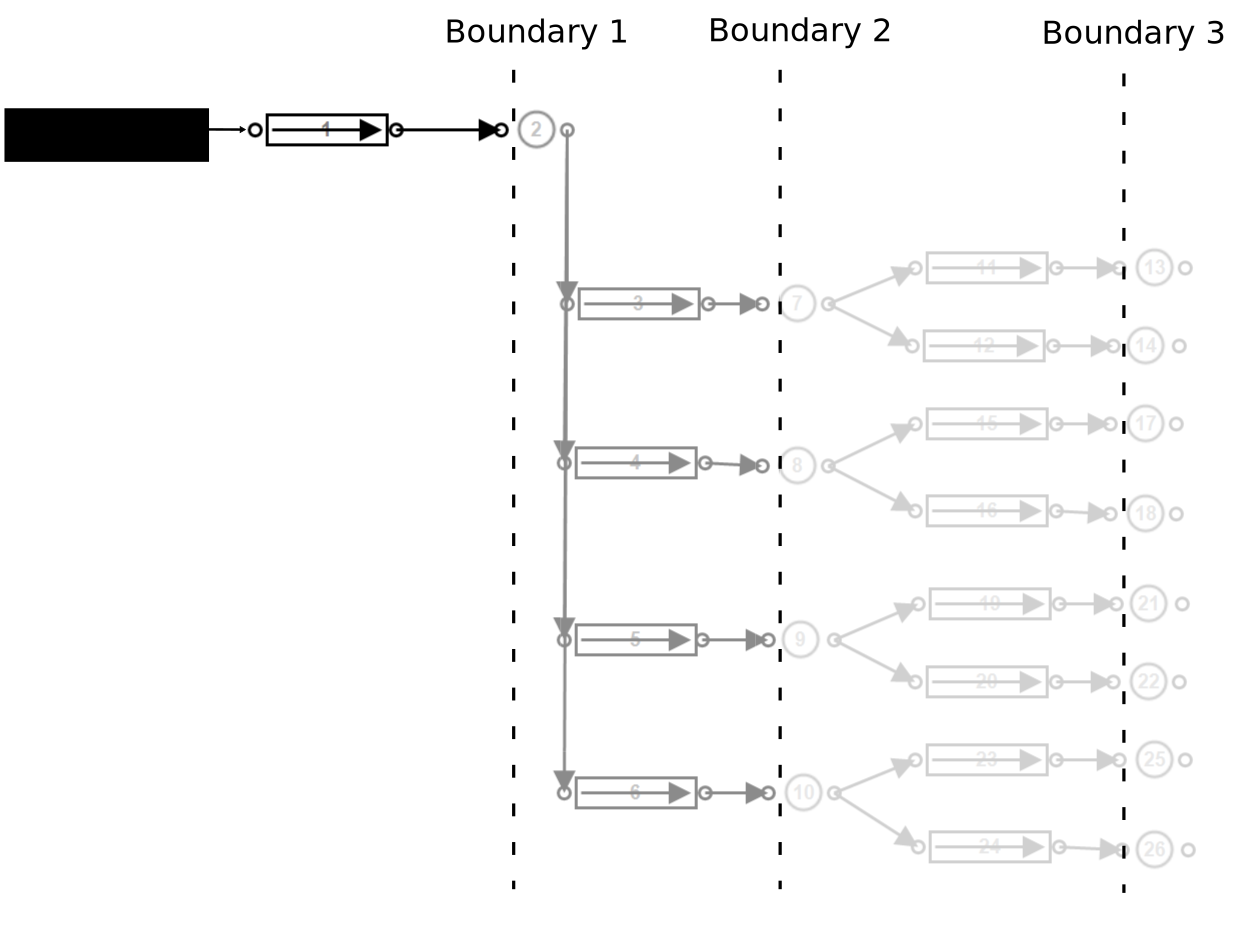
\includegraphics[width=0.88\textwidth]{Images/3/Detail.pdf}\hspace{0.05\textwidth}}
	 	\caption{Selecting boundaries for the simulation model}
	 	\label{fig: Sensitivity}
	 \end{figure}
	The process boundaries should be selected based on the input data available, the accuracy targets and the available time and resources. A more detailed model will allow more accurate simulation. However, it may take more time and resources to obtain the data required to calibrate the model. \Cref{fig: Sensitivity} contains an example of different boundary selection for the same system.
	\par
	Period and data step sizes of the simulation are just as important. The period or duration of the simulation should be determined to ensure that the effects of a scenario are fully tested. Previous studies commonly simulated a \enquote{typical} 24-hour period of operation, and most mining compressed air systems follow daily trends and patterns. Therefore, there is no need to simulate a longer period as day-to-day results would be very similar. A longer simulation may be required for cases where the system operation varies from day to day.
	\par 
	The simulation step size indicates the data resolution. A lower step size will result in a more accurate simulation of the system. However, the processing and data analysis may be affected. In this study, the smallest available step size\footnote{The minimum step size is determined from the logging interval of the input data instrumentation. For example, if all input data is logged at 10-minute intervals, the minimum step size would be 10 minutes.} was selected to ensure that the simulated results would achieve the desired precision. 
	\par 
	 Compressed air processes such as opening/closing valves or compressors stopping or starting may occur within minutes or seconds. Therefore, higher step sizes (30+ min.) may delay process changes. This delay makes replication of the system control more difficult, and it reduces simulation accuracy.
	\par
	A higher time-step resolution allows for more precise tuning of controllers and dynamic components. If input data is not available at the desired resolution, the data can be interpolated using the appropriate method. An example of the application of linear interpolation to increase the time-step resolution is shown in \Cref{fig: Inter}. However, incorrectly estimating the \enquote{in-between}  data value may adversely affect the simulation accuracy.
	
	\begin{figure}[h]
		\centering
		\fbox{\input{Graphs/3/inter/inter}}
		\caption{Interpolating input data to increase time-step resolution}
		\label{fig: Inter}
	\end{figure}
	\subsection{Model the air network components}
		\subsubsection{Ambient conditions}
		Ambient air conditions underground and on the surface changes the characteristics of the air, and affects the operation of the system. \Cref{fig: Ambient} shows the average summer air conditions. If no data is available for the specific simulation period, the conditions can be estimated by scaling this profile.
		\begin{figure}[h!]
			\centering
			\fbox{\input{Graphs/3/Ambient/Ambient}}
			\caption{Average summer surface ambient air conditions at a South African gold mine}
			\label{fig: Ambient}
		\end{figure}
		\par
		The assumption is made that underground conditions remain constant at each mining level. Pressure and temperature increase with depth as a result of auto compression and rock face temperature. Therefore, the conditions can be estimated using only the depth at each level.
		\subsubsection{Air pipes}
		Pressure losses occur over compressed air networks due to friction within the pipe. These losses should be taken into account in the simulation for large piping networks. A pipe model is used to account for these losses which are defined by the \textit{Darcy-Weisbach equation}\footnote{ B. Glenn, \enquote*{The Darcy–Weisbach Equation,}[Online] \url{https://bae.okstate.edu/faculty-sites/Darcy/DarcyWeisbach/Darcy-WeisbachEq.htm}, [Accessed 20-05-2017]}:
		$$\Delta P = \frac{f L \rho V^2}{2 D}$$
		Where the pressure difference $\Delta P $ is a function of:
		\begin{table}[h!]
			\centering
			\begin{tabular}{cl}
				\hline
				Parameter & Definition\\
				\hline
				$f$ & Friction coefficient \\
				$L$ & Pipe length ($m$) \\
				$D$ & Pipe diameter ($m$) \\
				$\rho$ & Air density ($kg/m^3$)\\	
				$V$ & Average velocity ($m/s$) \\	
				\hline
			\end{tabular} 
			\label{table: Darcy-Weisbach}
		\end{table}
		
		The pipe component may be used as a valve by controlling the open fraction between 0 and 1. Modelling the valve flow characteristics is discussed in \Cref{Controllers}-\textit{Controllers}.
		
		\subsubsection{Compressors}
		The following three compressor models were investigated, each with varying complexity. The models are:
		\begin{itemize}
			\item Air compressor model
			\item Dynamic compressor model
			\item Positive displacement compressor model
		\end{itemize} 
		The air compressor is a general, simplified model that requires minimal user input by making several assumptions. This model is useful when parameters for a compressor are not available. Alternatively, the air compressor model is ideal when doing a quick or preliminary simulation. However, it is not ideal for detailed simulations that require more precision.
		\par 
		The dynamic compressor components are more complex, and they take into account factors such as heat generated by the polytropic process and mechanical inefficiencies. Hence, the model can be used more accurately and for more complex simulations than the general compressor model. However, it should be noted that the dynamic compressor is simplified by several assumptions, for example, a constant efficiency at varying loads. 
		\par 	 
		For most scenarios, the dynamic compressor model is very suitable. The dynamic compressor is modelled by fitting a quadratic curve through three points of operation to obtain an equation for corrected mass flow as a function of the pressure ratio. This characteristic curve of a compressor (as shown in \Cref{fig: Compressor Curve}) can be accurately estimated even when only one data point is available by making approximations for the zero flow and pressure points on the curve.
		\par
		
		 Once the flow characteristics of the compressors are set, the efficiency and \gls{polyCof} parameters are calibrated such that the output power and air temperature match the actual or estimated outputs of the compressor.
		\par 
		\begin{figure}[h!]
			\centering
			\fbox{\input{Graphs/3/AproxCurve/AproxCurve}}
			\caption{Estimating the characteristic curve of a compressor by fitting a quadratic function to points of operation}
			\label{fig: Compressor Curve}
		\end{figure}
		Once the models have been accurately calibrated, the compressor component integrates into the air network in the arrangement shown in \Cref{fig: Compressor models}. The compressor is connected to the inlet air source via an inlet pipe and air node, and the rest of the network via an air node and outlet pipe. The additional pipe components allow the inlet and outlet conditions to be monitored and controlled in the simulation.
		\begin{figure}[h]
			\centering
			\fbox{\includegraphics[trim =-4cm 0 -4cm 0cm, width=0.98\textwidth]{Images/3/Compressors}}
			\caption{Integrating the compressor component into the simulation}
			\label{fig: Compressor models}
		\end{figure}		

		\subsubsection{Demand}
			A flow demand represents any air flow leaving the network. Flows leaving the network include any air-consuming equipment such as drills and agitators as well as losses by means of air leaks and open pipes. The air flow is dependent on pressure and the specific resistance to flow of the outlet. 
			\par 
			The resistance of the flow demand can be obtained using the inlet pressure, outlet pressure and flow. If the flow is not known, a reasonably accurate estimation can be made by calculating the expected flow from the size of the outlet. However, his estimation will affect the accuracy.
			\par
			 The air demand may vary throughout the day. For example, a mining section may utilise more machines during certain periods of the day. A schedule and flow profile is used to replicate this in the simulation. \Cref{fig: Demand component} shows how a calibrated air demand or leak is integrated into the simulation model on \gls{ptb}.
			\begin{figure}[h]
				\centering
				\fbox{\includegraphics[trim =-12cm 0.5cm -12cm 0.5cm, width=0.98\textwidth]{Images/3/AirDemand}}
				\caption{Implementing flow demands and leaks into the simulation} 
				\label{fig: Demand component}
			\end{figure}
		\subsubsection{Compressed air control}\label{Controllers}
			Simulation components require dynamic control to replicate the operation of the actual air network. Control is typically implemented on compressors and valves throughout the network to follow  set-points and schedules. It is important to not only include the controllers in the simulation but to replicate any nonlinearities, limitations and response delays related to specific types of control. Implementing these control factors will ensure that the model reacts in the same way as the actual network would, thus improving accuracy.
			\par 
			On a typical mine, a compressor's power output is controlled to ensure that the discharge pressure matches a specified  set-point. This control is achieved through either \glspl{vsd} (or \glspl{vfd}) and guide vane control. On \gls{ptb}, valve or compressor control can be replicated using a \gls{pi} controller as shown in \Cref{fig: Controller models}. For the control system models in \Cref{fig: Controller models}, outlet pressure is used as feedback to the compressor and a valve controller. 
			\par 
			
	\begin{figure}[h!]
		\centering
		\fbox{\includegraphics[trim =-4cm 0 -4cm 0cm, width=0.98\textwidth]{Images/3/Controller}}
		\caption[Control components in Process Toolbox]{Control components in Process Toolbox}
		\label{fig: Controller models}
	\end{figure}
		Guide vanes are most commonly used to control compressors in mining air systems. Guide vane control entails controlling the position of the inlet guide vane. The guide vane is opened or closed to control the compressors discharge pressure. Manipulating the guide vane position will affect the output power that the compressor puts into the system. 
		\par 
		\Cref{fig: Guide vane position} shows the relationship between power and guide vane position. A linear relation between guide vane position and compressor output can be used to estimate the effect of guide vane control. The model should take into account the minimum guide vane position limit that is typically set at around 40\% open. As illustrated in \Cref{fig: Guide vane position}, this control position maps to an output power for the compressor of about 60\% of maximum power. When more pressure is required than can be obtained with the guide vanes fully opened, another compressor is needed to operate. 
		\begin{figure}[h]
			\centering
			\fbox{\input{Graphs/1/GuideVainPosition/GuideVainPosition}}
			\caption{Modelling the compressor control from a guide vane\protect \footnotemark[1]}
			\label{fig: Guide vane position}
		\end{figure}
	
	\footnotetext[1]{Data recorded from a guide vane controlled compressor on a mine over a period of six months}
	
		In \gls{ptb}, the guide vane controller is modelled using a \gls{pi} controller. The non-linear limitations of guide vane control must be implemented in the controller. The control limitation is applied in the model by using a minimum control output limit that matches the minimum power reduction achieved by closing the guide vane to its minimum position. 
		\par 
		Mines make use of control valves at underground sections to adjust the pressure at individual mining stations independently \cite{Heyns2014Masters}. Controlling of valve components is performed similarly as control of the compressor components. \Cref{fig: Controller models} shows that the outlet pressure is used as feedback for a \gls{pi} controller. The control output is mapped to the valve fraction of a pipe component.

		\begin{figure}[h]
			\centering
			\fbox{\includegraphics[ width=0.8\textwidth]{Images/3/Valve.jpg}}
			\caption[An example of a compressed air control valve]{An example of a compressed air control valve\cite{van2015implementation}} 
			\label{fig: Control}
		\end{figure}
		\subsubsection{Compressed air after-cooling}
		The air compression process generates significant heat. Compressed air at high temperatures contains a significant amount of water vapour. After-coolers are installed on compressed air systems to prevent condensation in the air network, to improve the system capacity and to protect equipment from excessive heat \cite{schroeder2009energy}.
		\par 
		After-cooling reduces the output air temperature of the compressors. This cooling can affect the operation of the network. Hence, including after-cooling in the simulation model should improve accuracy.
		\par
		Modelling the after-cooling is achieved in \gls{ptb} using a heat transfer node at the outlet of the compressor component model. The heat transfer parameters shown in \Cref{table: After cooling inputs} should be calibrated such that the air temperature matches after-cooled air temperature measurements. An assumption of 40$^\circ$\gls{c} can be used if no measurements are available.
		\begin{table}
			\caption{The input parameters for the after-cooling simulation model}
			\centering
			\begin{tabular}{lll}
				\hline 
				Parameter \hspace{1cm} & Definition \hspace{4cm} & Unit \\
				\hline
				$A$ & The heat transfer area & $m^2$ \\
				$UA$ & Heat transfer coefficient & $kW/^{\circ} C$ \\
				$T_{amb}$ & Ambient air temperature & $^{\circ} C$ \\
				\hline
			\end{tabular}
		\label{table: After cooling inputs}
		\end{table}
	Depending on the accuracy requirement, after-cooling can be excluded from the simulation. Post after-cooling, compressed air is usually still warmer than ambient conditions. Air temperatures underground can be accurately matched by including heat transfer for compressed air pipelines.
	
	\subsection{Verify the simulation model}
	Based on the review of literature in \Cref{VerificationLit}, it was determined that \gls{mae} and the coefficient of determination are the most effective methods for measuring model accuracy. Therefore, both measures are utilised in the model verification in this study. These measures are obtained by comparing the major simulation outputs (total system power, flow and pressure) to actual data from the system. R-squared and \gls{mae} metrics are calculated by applying the applicable methodologies discussed in \Cref{VerificationLit}.	
	\par 
	For this study, the selected verification constraints were selected as : \\ {$r^2 > 0.9 $ and $ Err_{\%} < 5\% $}\\ 
	If these limits are met for the power, flow and pressure of the system, the model is considered accurate. As an extra measure, the relative error of the output for the minor model components should be $ > 85\%$ of the actual data. To obtain the true error of the model, instrumentation measurement error should be combined with the calculated simulation error.
	\par 
	Furthermore, periodically repeated simulations could be used to verify simulations more definitively. To perform the repeated simulation verification, the input variables should be updated for each new period. The output values of the simulation should then be compared with actual measurements. For each simulation, the verification constraints should be met.
		
	\subsection{Select simulation inputs}
		The inputs of a simulation are any parameters that do not remain static or follow the same profile in the day-to-day operation of the system. Examples of such parameters in a compressed air simulation are the following:
		\begin{itemize}
			\item Surface ambient conditions
			\item Machine operation schedules
			\item Air demands
			\item Operational changes
		\end{itemize} 
	Changing the simulation baseline period for a calibrated simulation should require only the updating of the input parameters. \Cref{fig: Compressor schedule} shows an example of a changing compressor schedule where an input parameter would need to be updated in the simulation.	

		\begin{figure}[h]
			\centering
			\fbox{\input{Graphs/3/CompSelection/CompSelection}}
			\caption{Example of two baseline periods, showing a changed compressor schedule}
			\label{fig: Compressor schedule}
		\end{figure}
	\subsection{Periodic simulation}	
		Periodic simulation refers to the repetition of simulations over subsequent periods to determine the sequential accuracy of the model. Sequential accuracy is important to verify that the model is valid in general and not just for a single period. This simulation will also indicate where operational changes have occurred as the simulation accuracy will be reduced.
		\par 
		The following procedure, as illustrated in \Cref{fig: PeriodicProcess}, was followed to implement periodic simulation: 
		\begin{itemize}
			\item Collect simulation input data periodically for each simulation interval
			\item Import input data series into the simulation model
			\item Execute/solve the simulation
			\item Export the output simulation values
			\item Compare output data with the systems actual operation and identify major discrepancies
			\item Trigger the process periodically
		\end{itemize}
	%%%%%%%%%%%%%
	\clearpage
		\begin{figure}[h]
			\centering
			\fbox{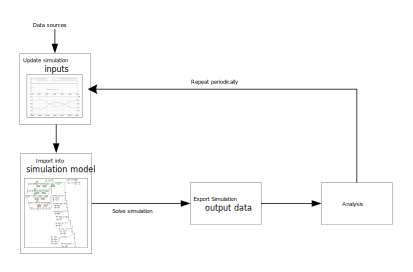
\includegraphics[trim =0.4cm 0.4cm 0.4cm 0.4cm,width=0.98\textwidth]{Graphs/4/PeriodicProcess/PeriodicProcess.pdf}}
			\caption{The periodic simulation process followed in this analysis}
			\label{fig: PeriodicProcess}
		\end{figure}
	
	\subsection{Summary}	
In this section, the subprocesses required for the development and verification of a simulation model were discussed. First, a method for selecting the model boundaries and parameters were reviewed, followed by a discussion on the modelling procedure for compressed air sub-components. The verification process and the selection of accuracy limits were next (see the analysis performed in section \Cref{VerificationLit}). The simulation input selection procedure was also reviewed and a procedure was provided for repeated/periodic simulation.

\section{Implement the simulation}
	\subsection{Preamble}
		Once a simulation has been developed and verified, the implementation of interventions and scenarios follows. In this section, the approach towards implementing the simulation methodology, and an analysis of interventions will be discussed.
	\subsection{Execute simulation scenarios}
		At this point, the simulation model has been verified using historical data. The verified output data series is now used as a baseline upon which interventions can be quantified. The simulation inputs of the model have now been adjusted to create the desired scenario. For example to create a scenario where a specific compressor is shut down over a period, the input schedule of the compressor is adjusted in the simulation model.
		\par
		The simulation is then executed, and this process is repeated for each of the scenarios. For each scenario, the desired output parameters must be exported for further analysis.

	\subsection{Quantify operational benefit}
		With the data for each of the simulated scenarios exported, the relative improvement compared with the baseline should now be quantified. This comparison is achieved by analysing the differences between the baseline and optimised data series as shown visually in \Cref{fig: Savings Power.}.
		\par 
		\begin{figure}[h]
			\centering
			\input{Graphs/3/savings/savings}
			\caption{Example of a baseline vs. optimised power comparison}
			\label{fig: Savings Power.}
		\end{figure} 
		\footnotetext[1]{Eskom, \enquote{2017/18 Tariffs and charges,} [Online] \url{http://www.eskom.co.za/CustomerCare/TariffsAndCharges/Pages/Tariffs_And_Charges.aspx}, [Accessed 28 June 2017]}
		
		For power data, the expected annual energy cost saving can be calculated using the average weekday energy saving and the tariff structure provided by Eskom. The energy supplier's weekday \gls{tou} tariffs for both the high demand (Jun -- Aug) and the low demand (Sep -- May) seasons are shown in \Cref{fig: Tariff}.
		\par 
		\begin{figure}[h]
			\centering
			\input{Graphs/3/tariff/tariff}
			\caption[Eskom's weekday TOU tariff structure]{Eskom's weekday time-of-use (TOU) tariff structure\protect \footnotemark[1]}
			\label{fig: Tariff}
		\end{figure}
		
		Estimating the cost benefit of improvements in pressure delivery is harder to quantify. Instead, the average pressure benefit for a period should be provided in kPa. For example, \enquote{The simulation indicated an $x$ MW saving with an additional pressure improvement of $y$ kPa during the drilling shift}.

		\subsection{Report results to the mine}
		Once the benefits for each simulated scenario have been calculated and quantified, the interventions should be prioritised according to the greatest benefit for the mine. The implementation costs and pay-back periods of the interventions can also be considered in this process.
		\par
		The results and recommendations should be submitted to responsible mine personnel in the form of a report (an example report is shown in \Cref{fig: Report example}). At this point, the process of implementation becomes the mine's responsibility. The mine may require further validation of the results through practical testing.
		\begin{figure}[h]
			\centering
			\fbox{\includegraphics[width=0.98\textwidth]{Images/3/ReportExample.pdf}}
			\caption{Example of a simulation report submitted to mine personnel}
			\label{fig: Report example}
		\end{figure}

	\subsection{Summary}
	This section discussed the implementation of the simulation procedure, which involves execution of the simulation scenarios, followed by the numerical calculation and quantification of energy cost savings and other benefits. Finally, a procedure for reporting findings to the mine is proposed.
\section{Conclusion}
The aim of Chapter 3 was to provide a methodology to develop compressed air simulations. The method was broken down into three steps:
\begin{enumerate}
	\item The \textbf{investigation} step involved obtaining and verifying data and information regarding the compressed air network. Processes to resolve scenarios where data can not be obtained were also suggested.
	\item In the next step, a procedure for \textbf{developing and verifying a simulation model} was provided. This procedure also described the selection of model and simulation parameters, the development of subcomponent models, as well as a verification procedure A methodology for repeated/periodic simulation was also provided.
	\item The final step involved the \textbf{execution} of the simulation followed by proposed methods to calculate, quantify and report the potential benefits of the simulated scenarios.
\end{enumerate}

%Chapter 4
\chapter{Results and validation}
\thispagestyle{empty}
\vspace{38em}
\hrulefill
\\
\enquote*{\textit{Quote.}} - Somebody\\
\newpage
\section{Introduction}
\section{Case study: Mine A \color{blue}(Kusasalethu)}
	\subsection{Preamble}
	\section{System investigation}
	
	\subsection{Model development}
	
	\subsubsection{Verification of baseline simulation}
	Verification of the model was done firstly by comparing the simulation outputs to actual measured values. To simplify the model, the actual measured pressure is temporarily used as set points for the compressors. This ensured that the pressure in the network is identical to that of the actual measured system as shown in figure \ref{fig: Verification Pressure kusasalethu}.
	\par 
	
	\begin{figure}[h]
		\centering
		\fbox{\input{Graphs/4/KusVerPressure/KusVerPressure}}
		\caption{Verifying Pressure}
		\label{fig: Verification Pressure kusasalethu}
	\end{figure}

 	With the pressure is set, the power and air flow outputs for components throughout the model were compared with their relative actual values. Figure \ref{fig: Verification Power kusasalethu} and figure \ref{fig: Verification flow kusasalethu} shows the comparison of the total power and flow of the system. The average error for these parameters was $1.08 \%$ and $1.80 \%$ respectively. This is regarded as acceptable error margin. 
 
	\begin{figure}[h]
		\centering
		\fbox{\input{Graphs/4/KusVerifyFlow/KusVerifyFlow}}
		\caption{Verifying flow.}
		\label{fig: Verification flow kusasalethu}
	\end{figure}
	\begin{figure}[h]
		\centering
		\fbox{\input{Graphs/4/KusVerPower/KusVerPower}}
		\caption{Verifying Power}
		\label{fig: Verification Power kusasalethu}
	\end{figure}
	Once all the power and flow parameters were regarded as correctly calibrated, the systems response to the actual pressure set-points was checked.
	
	\subsection{Scenario 1. Refuge bay simulation}
	Tested scenario where all excessive leaking valves are removed.
	Refuge bays savings 1MW E.E.
	
	\begin{figure}[h]
		\centering
		\fbox{\includegraphics[trim =-30cm 0 -20cm 0cm, width=\textwidth]{Images/A/RefBaySim}}
		\caption{Simulation layout for the refuge bay scenario.}
		\label{fig: Refuge bay layout}
	\end{figure}		
	
	
	
	
	\subsection{Scenario 2. Closing off levels/stopes}
	
	\subsection{Validation of results}
	\subsection{Summary}
\section{Case study: Mine B \color{blue}(Beatrix 123)}
	\subsection{Preamble}
	\subsection{Scenario 1. Compressor set points}
	\subsection{Scenario 2. Control valves set points}
	\subsection{Summary}
\section{Periodic simulation analysis}
	\subsection{Preamble}
	 Updating the inputs of a simulation periodically could be used to identify significant operational changes or when if the model parameters have drifted to a point where the model requires recalibration. This section will detail the results of an analysis into periodic simulation.
	 \subsection{Method of analysis}
	 
	 \subsection{Results}
	\subsection{Summary}
\section{Potential benefit for SA mines}
\section{Conclusion}
%Chapter 5
\chapter{Conclusion}
%\pagenumbering{gobble}
\vspace{38em}

\hrulefill
\\
%\enquote*{\textit{Quote.}} - Somebody\\
\newpage
		\section{Preamble}
		Chapter 5 serves as a conclusion for this dissertation. An overview of the complete dissertation will be provided. This overview will summarise the work done in the proceeding chapters. The limitations of the study will then be discussed. This will lead to discussion and recommendations for future work that can be done in the field.
	 \section{Dissertation overview}
	 The South African mining sector is currently facing significant challenges that pose a risk to profitability of the industry. A pivotal challenge that faces the industry is that of rising operational costs. Energy costs pertain a significant portion of the cost increases as energy tariff increases have constantly surpassed inflation over the passed 10 years.
	 \par
	 Compressed air systems consume the largest portion of energy used in a mine. Compressed air has also been shown to be largely inefficient. It is there for reasoned that the largest energy impact can be achieved through compressed air interventions.
	 \par 
	 Energy intervention in mining compressed air have been performed in the passed. However, compressed air simulation has not been used to its full potential. Using new computer modelling and simulation tools for compressed air systems, the detailed effects of interventions can be identified with minimal risk. This will lead to further energy and cost reductions as well as other potential improvements for a mines operation.
	 \par 
	 An review of background and literature was performed. The purpose of the review was to provide background on mining compressed air networks and to evaluate literature in pertaining to compressed air energy interventions, simulation usage the mining industry and specifically simulation usage in compressed air systems.
	 \par 
	 Using the findings in from the literature review, a methodology was developed for compressed air simulation. The methodology describes the a simulation procedure in three steps summarised as: investigate the system, develop a simulation model and execute the simulation scenarios.
	 \par 
	 The simulation methodology was then validated through implementationon case studies. The studies were implemented on two separate mine compressed air systems. A full system investigation was performed in each study. From the data and understand obtained for the investigation, simulation models were developed for both systems.
	 \par
	 \emph{...Incomplete....}
	 \section{Limits of this study}
	 \section{Recommendations for future studies}
	 
	 
%Appendices
\begin{appendices}
\chapter{A}

\chapter{B}
\end{appendices}

\bibliographystyle{plain}
\bibliography{Bibliography}

\end{document}